
\chapter{系统框架}
\label{chap:framework}
\section{整体框架介绍}
\label{sec:wholeframework}
本文的主要工作在于搭建一个自动的网页模板抽取系统。系统主要分为三个模块:“预处理
模块”,“网页聚类模块”和“网页模板生成和内容提取模块”。从输入的网页集合开始,
依次经过以上三个模块,生成模板后用于提取新的网页中的信息,然后将提取的信息以XML的
格式输出成格式化数据。

整体的框架示意如\reffig{framework:fig:framework}所
示,\reffig{framework:fig:framework}包括了系统的训练和测试。其中,系统训练的输入
是目前已经从互联网上所获得的网页集合,训练的输出为这些网页集合所对应的模板,这部
分系统是离线的。系统的测试输入为新的网页,测试的输出为XML格式的数据,这部分是在线
的。

\begin{figure}
  \centering
  \begin{tikzpicture}[scale=.58,transform shape,
    font=\large,
    io/.style={fill=black!30, text width=3cm, minimum size=1cm,align=center,draw=black},
    submodule/.style={fill=cyan!80, text width=3cm, minimum size=1cm, rounded corners,align=center,draw=black},
    bold arrow/.style={very thick, >=triangle 90},
    input arrow/.style={single arrow, minimum width=5mm, minimum height=0.8cm, draw},
    mylabel/.style={dotted, draw}
    ]    
    \node (input) [io] {输入网页};
    \node (input-arrow) [below=1mm of input, input arrow, shape border rotate=270]{};
    \node (m1-1) [submodule, below=4mm of input-arrow]{过滤无用网页};
    \node (m1-2) [submodule, below=5mm of m1-1]{简化HTML文档} edge[<-] (m1-1);
    \node (m2-1) [submodule, below=1.2cm of m1-2]{结构相似度计算};
    \draw [<-, bold arrow] (m2-1) -- (m1-2);
    \node (m2-2) [submodule, below=5mm of m2-1]{网页聚类} edge[<-] (m2-1);
    \node (m3-1) [submodule, below=1.2cm of m2-2]{模板生成};
    \draw [<-, bold arrow] (m3-1) -- (m2-2);
    \node (m3-2) [submodule, below=5mm of m3-1]{内容抽取} edge[<-] (m3-1);
    \node (new-input-arrow)[left=5mm of m3-2, input arrow]{};
    \node (new-input) [io, left=2mm of new-input-arrow]{新的网页输入};
    \node (output) [io, below=of m3-2]{XML输出};
    \draw [<-, bold arrow] (output) -- (m3-2);
  \begin{pgfonlayer}{background}
    \tikzset{module/.style={inner sep=1em, fill=white, fill=green!30, rounded corners}};
    \node (m1)[module, fit=(m1-1) (m1-2)]{};
    \node (m1-name) [right=5mm of m1]{\Large{预处理模块}};
    \node (m2)[module, fit=(m2-1) (m2-2)]{} [below=of m1];
    \node (m2-name) [right=5mm of m2]{\Large{网页聚类模块}};
    \node (m3)[module, fit=(m3-1) (m3-2)]{} [below=of m2];
    \node (m3-name) [right=5mm of m3] {\Large{模板生成和内容提取模块}};
  \end{pgfonlayer}  
\end{tikzpicture}
  \caption{系统整体框架示意}
  \label{framework:fig:framework}
\end{figure}

以下将逐个介绍各个模块的总体设计。
\section{预处理模块}
\label{sec:filterintro}
预处理模块主要以下分为两个子模块:过滤无用网页和简化HTML文档。
\subsection{过滤无用网页}
\label{sec:filterintro-useless}
我们获得的网页数据主要分为以下几种:目录页、详细页、404及其他错误页。在我们的实验
中,我们只关心详细页的集合,因此,需要首先过滤掉目录页和错误页等无用的网页。

这部分要求要有较快的运行速度,因此不需要设计非常复杂的算法,主要通过设置一些简单
的规则去对原始的网页集合进行过滤。通过观察,我们主要采取了以下这些策略:
\begin{itemize}
\item 404及其他类似的错误页可以通过一些关键字如{404 Not
    Found}或者{Server Error}等进行辨别。通常这些错误页的文档都很简单,长度
  很短,因此还可以通过设置长度阈值将其过滤;这样还可以将一些无用的太短的文档同时
  去除。
\item 大部分目录页的URL和详细页的URL有明显区别。比如对于新浪博客来说,详细页的
  URL都以{.html}结尾,而目录页则没有。例如以下两个URL:
http://blog.sina.com.cn/u/1439351555\\
http://blog.sina.com.cn/s/blog\_55cac30301016yb1.html\\
第一个URL对应的是某个博主的文章目录,第二个URL则是该博主的某篇文章。因此只需要通
过正则表达式匹配的方式即可将目录页过滤。其他网站也有类似这样的规则,我们只需要在
实验前针对每个网站提前设置好规则进行过滤即可。由于每个网站每种特定的网页只需要指
定一种规则,人工的工作量并不大。
\item 为了实验的完备性和对一些特殊的网站进行处理,比如可能存在某些网站,目录页
  的URL和详细页的URL在模式没有太大的区别,或者人工设置规则的办法太麻烦了,我们的
  系统中也实现了通过网页的特征过滤详细页的机制。注意到目录页的作用主要是给用户提
  供进入各个详细页的入口,因此目录页的HTML文档的主要部分是由列表环
  境{<ul>}或{<ol>}中的列表项{<li>}及其包含的超链接标
  签{<a>}组成。\reffig{framework:fig:baidunews}是简化后的百度新闻目录
  页HTML代码的一部分\footnote{来源:2013年6月9日15时的news.baidu.com页面}。我们提
  取出网页中的所有{<li>}标签中的{<a>}标签,计算这些{<a>}标签
  的文本内容占网页所有文本内容的比重,超过一定的阈值则判定为目录页。由于这种方法
  比上述使用简单规则的办法要慢许多,因此在系统中我们将优先使用规则的方法对目录页
  进行过滤。
\end{itemize}
\begin{figure}
  \centering
  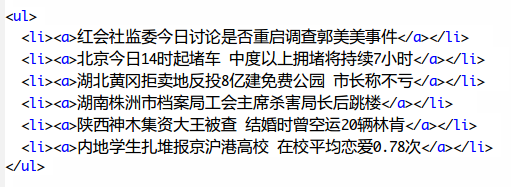
\includegraphics[width=0.5\textwidth]{framework02/baidunews}
  \caption{简化的百度新闻目录页的一部分HTML代码}
  \label{framework:fig:baidunews}
\end{figure}

通过这些策略将目录页和错误页过滤完以后,我们可以得到网页的详细页集合,将其作为下
一个子模块的输入。
\subsection{简化HTML文档}
我们将分多个步骤对HTML文档进行简化。

第一步是去除无用的标签。这些标签有以下特点:
\begin{enumerate}
 \item\label{item:1} 与网页模块无关。去除这些标签时,可以将标签本身及标签的内容一同去掉。比如
  {<script>}、{<link>}、{<style>}等。
\item\label{item:2} 通常是深层次的HTML文档的节点,用于控制格式,在模板中意义不大。
  去除这些标签时只取出标签本身,保留标签所包含的内容。比
  如{<br/>}、{<p>}、{<strong>}、{<em>}等。
\item\label{item:3} 我们在实验中不考虑非文本标签,因此将{<img>}、
  {<audio>}等直接去除。
\item\label{item:4} 最后是去除一些在模板中变化很大的太复杂的标签,典型的是表格相
  关的一些标签,包
  括{<table>}、{<th>}、{<tr>}、{<td>}等。
\end{enumerate}

接下来我们把每个HTML文档都解析成DOM Tree。DOM Tree的构建速度比较慢,在解析时需要
将整个HTML同时载入内存,占用较多的内存资源,可能导致我们在需要处理的数据量较大时
会出现一定的问题。去除这些无用标签可以加快HTML解析成DOM Tree的速度,减小内存占用,
也减小了后续的模板聚类和模板检测中的噪音,是很有必要的。

第二步是对解析好的DOM Tree进行简化。由于在树形结构上做相关的操作较为复杂,我们首
先将树形结构转化为更便于处理的序列形式。具体地,我们采用先序遍历的方式,将DOM
Tree转化成一个标签序列,为了可以还原成原始的DOM Tree,我们在遍历的同时在每个节点
处保存了该节点的深度信息。对于\reffig{framework:fig:html}所示的HTML文档,解析成
的DOM Tree如\reffig{framework:fig:domtree}所示,如果每个标签采用{标签名+深
  度}的表示方法,则我们采用先序遍历方式可以得到该DOM Tree对应的序列
为:{<html0><body1><div2><a3><p3><div2>}。先序遍历的优点在于可以保证每个子
树的所有节点在序列中的位置是连续的,且根节点位于这段连续子序列的起始处。比如以第
一个{<div>}标签为根的子树在遍历得到的序列中对应的序列
为{<div2><a3><p3>},根节点{<div2>}位于子序列的起始位置。这些特点对
于后续的处理有很大的帮助。

第三步是对HTML文档中重复出现的记录进行检测,去掉重复的多余的部分,从而用更简单的
方式表示原文档。我们将DOM Tree的某个子树成为一个“记录”。由于HTML模板中动态生成
的部分中可能包含大量重复的模式,比如\reffig{intro:fig:django-hard}所示的Django模
板,其中的{news.comments}可能包含不定数目的元素,在比较由这个模板生成的两
个不同网页的时候,应该将其中数目可能不一样的{<li>}的结构视为一样,否则将对
后续的处理造成较大的误差。在网页的生成中,这种重复模式是大量存在的,因此,检测网
页中的重复记录并做相应的简化是预处理过程中最重要的一个部分,我们将在
第~\ref{chap:suffixtree}章中详细介绍。
\begin{figure}
  \begin{minipage}[t]{0.5\linewidth}
  \centering
  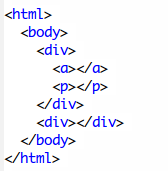
\includegraphics[width=0.5\textwidth]{framework02/framework-html}
  \caption{一个简单的HTML文件}
  \label{framework:fig:html}
\end{minipage}
\begin{minipage}[t]{0.5\linewidth}
  \centering
  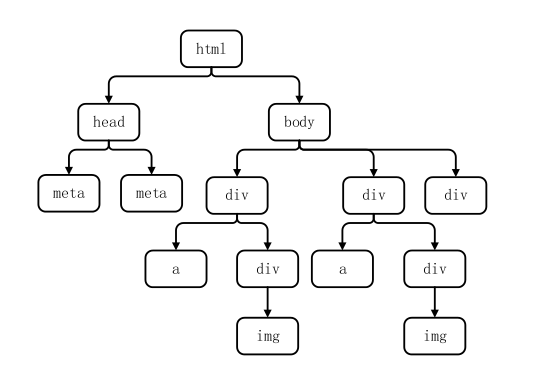
\includegraphics[width=0.5\textwidth]{framework02/domtree}
  \caption{\reffig{framework:fig:html}对应的DOM Tree}
  \label{framework:fig:domtree}
\end{minipage}
\end{figure}
\section{网页聚类模块}
\label{sec:clusterintro}
这个模块包含两个主要的子模块:计算网页结构相似度和实现网页聚类算法。

通过网页的预处理模块,我们将得到一个简化的由DOM Tree先序遍历得到的序列,其中不包
含重复的记录。为了能够进行聚类,我们首先需要计算每个文档之间的结构相似度。这里我
们采用的是基于最长公共子序列(Longest Common Sequence)的方法,简称LCS。实际上,我们
整个工作中与序列处理相关的工作很多都将基于LCS,包括后面的模板生成和内容提取模块。
我们将对每两个文档都计算一次LCS,得到文档之间的结构相似度,将其用于后续的聚类。

在聚类子模块,有几个特点值得我们注意:
\begin{itemize}
\item 网页中的模板个数即最终聚类的个数事先是不知道的,因此我们不能采用一些类似
  于K-means等需要预先设定聚类的个数的算法。
\item 网页数量很大,需要有较快的执行速度。
\item 我们可以利用的信息只有网页文档两两之间的结构相似度。
\end{itemize}

我们将采用简单的层次聚类的方法,通过设置阈值的方法控制聚类的类别个数。这个模块的
具体实现将在第~\ref{chap:cluster}章中详细介绍。
\section{模板生成和内容提取模块}
\label{sec:templateintro}
这个模块是本次实验中最主要的部分,包括两个子模块:模板生成和内容提取。

在模板生成子模块中,我们将从之前聚好的类中提取出每个类对应的模板。模板的提取将仍
然基于DOM Tree先序遍历得到的序列和LCS,并利用无监督的方法来进行构建。这个子模块输
出的模板将作为整个系统的训练模块的输出。

为了能够从网页中提取出我们所需要的部分,我们还需要人工对模板中的某些部分指定语义,
比如对于新闻来说,模板中的哪些部分将对应新闻标题、正文、评论等。由于模板的数量不
会很多,这部分的工作量不会很大。

内容提取子模块将利用之前训练得到的聚类信息和模板,选择合适的模板从新的网页中提取
出我们需要的信息,并将这个信息以XML格式输出成结构化的数据。

这个模块我们将在第~\ref{chap:template}章中进行详细介绍。
\section{本章小结}
\label{sec:summaryframework}
本章首先简单介绍了系统的整体框架,然后分别对每个模块的总体设计进行了说明。其中我
们重点介绍了预处理模块中除了重复记录检测子模块以外的部分,其他概述的部分,如重复
记录的检测,网页的聚类,模板生成和内容提取等,我们将在后续章节中一一详细介绍。

%%% Local Variables: 
%%% mode: latex
%%% TeX-master: "../main"
%%% End: 
